% Options for packages loaded elsewhere
\PassOptionsToPackage{unicode}{hyperref}
\PassOptionsToPackage{hyphens}{url}
\PassOptionsToPackage{dvipsnames,svgnames,x11names}{xcolor}
%
\documentclass[
  ignorenonframetext,
  aspectratio=169,
]{beamer}
\usepackage{pgfpages}
\setbeamertemplate{caption}[numbered]
\setbeamertemplate{caption label separator}{: }
\setbeamercolor{caption name}{fg=normal text.fg}
\beamertemplatenavigationsymbolshorizontal
% Prevent slide breaks in the middle of a paragraph
\widowpenalties 1 10000
\raggedbottom
\setbeamertemplate{part page}{
  \centering
  \begin{beamercolorbox}[sep=16pt,center]{part title}
    \usebeamerfont{part title}\insertpart\par
  \end{beamercolorbox}
}
\setbeamertemplate{section page}{
  \centering
  \begin{beamercolorbox}[sep=12pt,center]{part title}
    \usebeamerfont{section title}\insertsection\par
  \end{beamercolorbox}
}
\setbeamertemplate{subsection page}{
  \centering
  \begin{beamercolorbox}[sep=8pt,center]{part title}
    \usebeamerfont{subsection title}\insertsubsection\par
  \end{beamercolorbox}
}
\AtBeginPart{
  \frame{\partpage}
}
\AtBeginSection{
  \ifbibliography
  \else
    \frame{\sectionpage}
  \fi
}
\AtBeginSubsection{
  \frame{\subsectionpage}
}

\usepackage{amsmath,amssymb}
\usepackage{iftex}
\ifPDFTeX
  \usepackage[T1]{fontenc}
  \usepackage[utf8]{inputenc}
  \usepackage{textcomp} % provide euro and other symbols
\else % if luatex or xetex
  \usepackage{unicode-math}
  \defaultfontfeatures{Scale=MatchLowercase}
  \defaultfontfeatures[\rmfamily]{Ligatures=TeX,Scale=1}
\fi
\usetheme[]{Hannover}
\usecolortheme{rose}
\usepackage[]{libertinus}
\ifPDFTeX\else  
    % xetex/luatex font selection
\fi
% Use upquote if available, for straight quotes in verbatim environments
\IfFileExists{upquote.sty}{\usepackage{upquote}}{}
\IfFileExists{microtype.sty}{% use microtype if available
  \usepackage[]{microtype}
  \UseMicrotypeSet[protrusion]{basicmath} % disable protrusion for tt fonts
}{}
\makeatletter
\@ifundefined{KOMAClassName}{% if non-KOMA class
  \IfFileExists{parskip.sty}{%
    \usepackage{parskip}
  }{% else
    \setlength{\parindent}{0pt}
    \setlength{\parskip}{6pt plus 2pt minus 1pt}}
}{% if KOMA class
  \KOMAoptions{parskip=half}}
\makeatother
\usepackage{xcolor}
\newif\ifbibliography
\setlength{\emergencystretch}{3em} % prevent overfull lines
\setcounter{secnumdepth}{-\maxdimen} % remove section numbering


\providecommand{\tightlist}{%
  \setlength{\itemsep}{0pt}\setlength{\parskip}{0pt}}\usepackage{longtable,booktabs,array}
\usepackage{calc} % for calculating minipage widths
\usepackage{caption}
% Make caption package work with longtable
\makeatletter
\def\fnum@table{\tablename~\thetable}
\makeatother
\usepackage{graphicx}
\makeatletter
\def\maxwidth{\ifdim\Gin@nat@width>\linewidth\linewidth\else\Gin@nat@width\fi}
\def\maxheight{\ifdim\Gin@nat@height>\textheight\textheight\else\Gin@nat@height\fi}
\makeatother
% Scale images if necessary, so that they will not overflow the page
% margins by default, and it is still possible to overwrite the defaults
% using explicit options in \includegraphics[width, height, ...]{}
\setkeys{Gin}{width=\maxwidth,height=\maxheight,keepaspectratio}
% Set default figure placement to htbp
\makeatletter
\def\fps@figure{htbp}
\makeatother
% definitions for citeproc citations
\NewDocumentCommand\citeproctext{}{}
\NewDocumentCommand\citeproc{mm}{%
  \begingroup\def\citeproctext{#2}\cite{#1}\endgroup}
\makeatletter
 % allow citations to break across lines
 \let\@cite@ofmt\@firstofone
 % avoid brackets around text for \cite:
 \def\@biblabel#1{}
 \def\@cite#1#2{{#1\if@tempswa , #2\fi}}
\makeatother
\newlength{\cslhangindent}
\setlength{\cslhangindent}{1.5em}
\newlength{\csllabelwidth}
\setlength{\csllabelwidth}{3em}
\newenvironment{CSLReferences}[2] % #1 hanging-indent, #2 entry-spacing
 {\begin{list}{}{%
  \setlength{\itemindent}{0pt}
  \setlength{\leftmargin}{0pt}
  \setlength{\parsep}{0pt}
  % turn on hanging indent if param 1 is 1
  \ifodd #1
   \setlength{\leftmargin}{\cslhangindent}
   \setlength{\itemindent}{-1\cslhangindent}
  \fi
  % set entry spacing
  \setlength{\itemsep}{#2\baselineskip}}}
 {\end{list}}
\usepackage{calc}
\newcommand{\CSLBlock}[1]{\hfill\break\parbox[t]{\linewidth}{\strut\ignorespaces#1\strut}}
\newcommand{\CSLLeftMargin}[1]{\parbox[t]{\csllabelwidth}{\strut#1\strut}}
\newcommand{\CSLRightInline}[1]{\parbox[t]{\linewidth - \csllabelwidth}{\strut#1\strut}}
\newcommand{\CSLIndent}[1]{\hspace{\cslhangindent}#1}

\makeatletter
\@ifpackageloaded{caption}{}{\usepackage{caption}}
\AtBeginDocument{%
\ifdefined\contentsname
  \renewcommand*\contentsname{Table of contents}
\else
  \newcommand\contentsname{Table of contents}
\fi
\ifdefined\listfigurename
  \renewcommand*\listfigurename{List of Figures}
\else
  \newcommand\listfigurename{List of Figures}
\fi
\ifdefined\listtablename
  \renewcommand*\listtablename{List of Tables}
\else
  \newcommand\listtablename{List of Tables}
\fi
\ifdefined\figurename
  \renewcommand*\figurename{Figure}
\else
  \newcommand\figurename{Figure}
\fi
\ifdefined\tablename
  \renewcommand*\tablename{Table}
\else
  \newcommand\tablename{Table}
\fi
}
\@ifpackageloaded{float}{}{\usepackage{float}}
\floatstyle{ruled}
\@ifundefined{c@chapter}{\newfloat{codelisting}{h}{lop}}{\newfloat{codelisting}{h}{lop}[chapter]}
\floatname{codelisting}{Listing}
\newcommand*\listoflistings{\listof{codelisting}{List of Listings}}
\makeatother
\makeatletter
\makeatother
\makeatletter
\@ifpackageloaded{caption}{}{\usepackage{caption}}
\@ifpackageloaded{subcaption}{}{\usepackage{subcaption}}
\makeatother
\ifLuaTeX
  \usepackage{selnolig}  % disable illegal ligatures
\fi
\usepackage{bookmark}

\IfFileExists{xurl.sty}{\usepackage{xurl}}{} % add URL line breaks if available
\urlstyle{same} % disable monospaced font for URLs
\hypersetup{
  pdftitle={Open Science},
  pdfauthor={Usman Afzali, PhD - Postdoctoral Fellow and Lecturer},
  colorlinks=true,
  linkcolor={Maroon},
  filecolor={Maroon},
  citecolor={Blue},
  urlcolor={Blue},
  pdfcreator={LaTeX via pandoc}}

\title{Open Science}
\author{Usman Afzali, PhD - Postdoctoral Fellow and Lecturer}
\date{2024-07-25}
\institute{University of Canterbury}
\logo{
\includegraphics{mds.png}}

\begin{document}
\frame{\titlepage}

\begin{frame}{Outline}
\phantomsection\label{outline}
\begin{itemize}
\tightlist
\item
  Scientific publishing
\item
  Open science
\item
  Preregistration
\item
  Conclusion
\end{itemize}
\end{frame}

\section{Scientific Publishing}\label{scientific-publishing}

\begin{frame}{The Evolution of Scientific Publishing}
\phantomsection\label{the-evolution-of-scientific-publishing}
\begin{itemize}[<+->]
\tightlist
\item
  Philosophical Transactions of the Royal Society (1655) by Henry
  Oldenburg. (\url{https://royalsocietypublishing.org/rsta/about})
\item
  Also, Journal des Sçavans (1665)
  (\url{https://en.wikipedia.org/wiki/Journal_des_sçavans}).
\item
  Nature (1869) by Sir Joseph Norman Lockyer
  (\url{https://www.nature.com/nature-portfolio/about}) (\emph{IF =
  54.4}).
\item
  19th Century: Growth of specialized journals.
\item
  20th Century: Rise of electronic publishing and faster dissemination
  and broader access through digital means
\end{itemize}
\end{frame}

\begin{frame}{Paywalls and Access to Scientific Articles}
\phantomsection\label{paywalls-and-access-to-scientific-articles}
\begin{itemize}[<+->]
\tightlist
\item
  Initially, published by scientific societies or university presses
\item
  Funded through memberships, subscriptions, or institutional support
\item
  Commercial publishing: subscription fees and profit motivation
\item
  Open Access journals
\item
  Hybrid journals
\item
  Some examples: \href{https://onlinelibrary.wiley.com}{Wiley},
  \href{https://www.taylorfrancis.com}{Routldeg/Taylor and Francis},
  \href{https://www.elsevier.com/products/sciencedirect/journals}{Elsevier},
  \href{https://www.nature.com/nature/journal-impact}{Nature},
  \href{https://www.apa.org/pubs/journals}{APA}.
\end{itemize}
\end{frame}

\begin{frame}{Questionable Research Practices (QRPs)}
\phantomsection\label{questionable-research-practices-qrps}
\begin{itemize}[<+->]
\tightlist
\item
  False positive psychology (Simmons, Nelson, and Simonsohn 2011)
\item
  Researchers degrees of freedom
\item
  Data manipulation, selective reporting, lack of transparency (e.g., in
  terms of excluding outliers)
\item
  Choosing the DV, choosing sample size, covariates, reporting a subset
  only
\end{itemize}
\end{frame}

\begin{frame}{Listening to ``Why I'm Sixty-Four'' makes you younger}
\phantomsection\label{listening-to-why-im-sixty-four-makes-you-younger}
\begin{center}
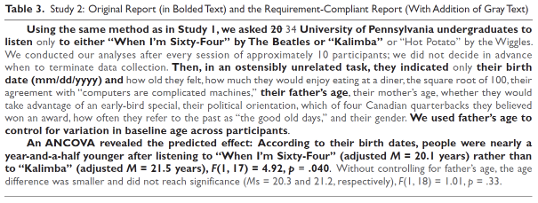
\includegraphics[width=0.8\textwidth,height=\textheight]{figs/p-Hacking.png}
\end{center}
\end{frame}

\begin{frame}{\emph{p}-Hacking}
\phantomsection\label{p-hacking}
\begin{itemize}[<+->]
\tightlist
\item
  Manipulation of data analysis or reporting practices to find
  statistically significant results
\item
  Inflates the likelihood of finding false positives, undermines the
  reliability of research
\end{itemize}
\end{frame}

\begin{frame}{Possible reasons for \emph{p}-Hacking}
\phantomsection\label{possible-reasons-for-p-hacking}
\begin{itemize}[<+->]
\tightlist
\item
  \textbf{Researcher's Intent:} Desire to publish significant findings.
\item
  \textbf{Ambiguity in Data Analysis:} Lack of clear analytical plans.
\item
  \textbf{Lack of Pre-planning:} Not specifying methods before data
  collection.
\end{itemize}
\end{frame}

\begin{frame}{Changing the false positive rate}
\phantomsection\label{changing-the-false-positive-rate}
\begin{center}
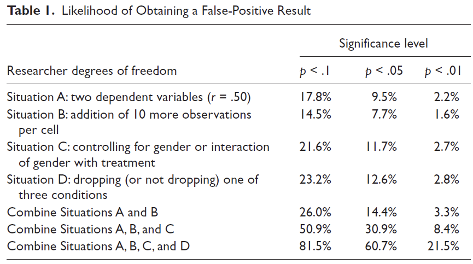
\includegraphics[width=0.8\textwidth,height=\textheight]{figs/p-Hacking-table.png}
\end{center}
\end{frame}

\begin{frame}{HARKing}
\phantomsection\label{harking}
\begin{itemize}[<+->]
\tightlist
\item
  Hypothesizing After the Results are Known
\item
  Presenting a \emph{post hoc} hypothesis as if it were an \emph{a
  priori} hypothesis
\item
  Dataset: significant correlation between X and Y, \emph{p} = .02
\item
  What are the chances of finding this correlation in this dataset?
\item
  HARKing ruins the meaning of \emph{p}-values
\end{itemize}
\end{frame}

\begin{frame}{Why would one engage in QRP's?}
\phantomsection\label{why-would-one-engage-in-qrps}
\begin{itemize}[<+->]
\tightlist
\item
  Pressure to Publish (``Publish or Perish'')
\item
  Career advancement
\item
  Research funding
\item
  Some examples: \emph{p}-Hacking, HARKing, selective reporting, data
  fabrication/falsification, inadequate reporting of methods and
  procedures, publication bias, over-interpretation of results
\end{itemize}
\end{frame}

\begin{frame}{Avoiding QRP's}
\phantomsection\label{avoiding-qrps}
\begin{center}
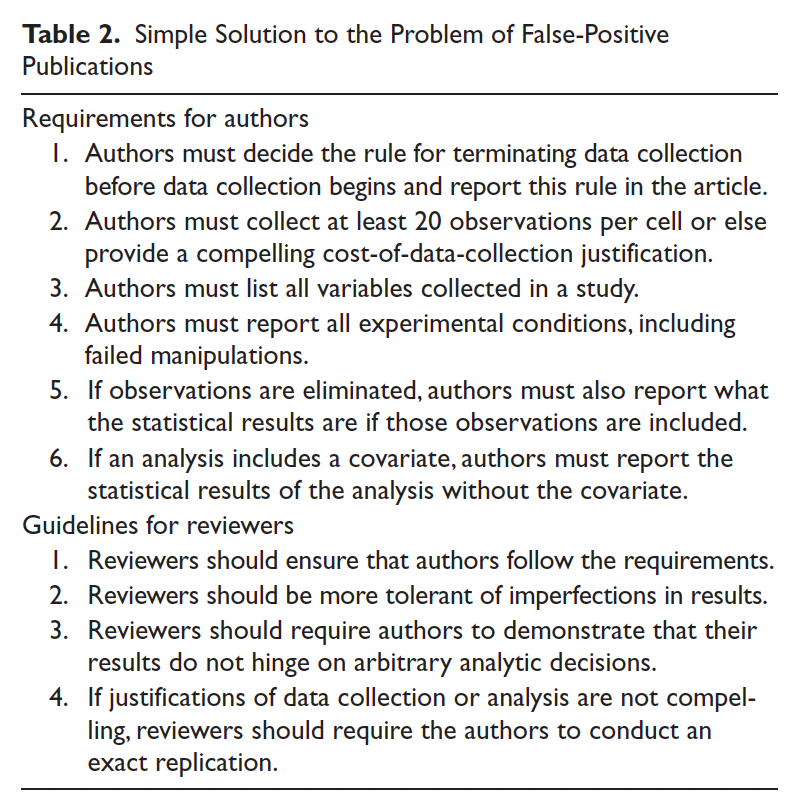
\includegraphics[width=0.5\textwidth,height=\textheight]{figs/avoid-qrp.png}
\end{center}
\end{frame}

\section{Open Science}\label{open-science}

\begin{frame}{}
\phantomsection\label{section}
\begin{itemize}[<+->]
\tightlist
\item
  Involves practices that make research processes and outputs more
  transparent and accessible
\item
  Enhances reproducibility, accountability, and collaboration in
  research
\item
  Premise: Science works best in sunlight
\item
  Science paid for by public, given to journals, sold back to public
\item
  Publication model relies on universities paying for access to journals
\item
  Science should be publicly available
\item
  Preprints (PsyArXiv: \url{https://osf.io/preprints/psyarxiv})
\item
  Open access/hybrid journals
\end{itemize}
\end{frame}

\begin{frame}{}
\phantomsection\label{section-1}
\begin{center}
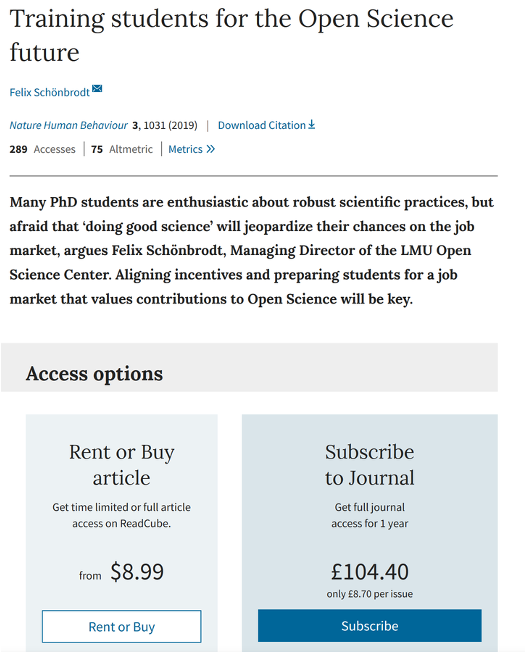
\includegraphics[width=0.7\textwidth,height=\textheight]{figs/paid-os.png}
\end{center}
\end{frame}

\begin{frame}{Open Materials}
\phantomsection\label{open-materials}
\begin{itemize}
\tightlist
\item
  Journal articles have word limits, often lack key details
\item
  Unpublished studies left in file drawer -- generally, published on
  OSF, or linked it from PsyArXiv to OSF
\end{itemize}
\end{frame}

\begin{frame}{Open Data}
\phantomsection\label{open-data}
\begin{itemize}
\tightlist
\item
  Allows researchers to check for mistakes, fraud
\item
  Be careful with confidentiality and privacy
\item
  Enhances potential for meta-analysis, re-analysis
\end{itemize}
\end{frame}

\begin{frame}{Preregistration}
\phantomsection\label{preregistration}
\begin{itemize}
\tightlist
\item
  Design, analyses pre-planned
\item
  Preregistration = writing up your hypotheses, conditions, data
  analytic plan, etc.
\item
  Prevents \emph{p}-hacking, HARKing
\item
  Does not prevent fraud
\end{itemize}
\end{frame}

\begin{frame}{Registered Reports}
\phantomsection\label{registered-reports}
\begin{itemize}
\tightlist
\item
  Peer-review \emph{before} data collection: e.g.,
  \url{https://osf.io/nru4x/?view_only=bc189174a1cf4ca8b1dc83cf7967cd9e}
\end{itemize}
\end{frame}

\begin{frame}{}
\phantomsection\label{section-2}
Open Access (OA) refers to making research outputs freely available
online, without subscription or payment barriers.

The Open Access movement advocates for free and unrestricted access to
research publications. Many researchers and institutions support this
model, arguing that publicly funded research should be freely available
to everyone. There are various Open Access models, including Gold Open
Access (where authors or institutions pay publication fees) and Green
Open Access (where authors deposit preprints or postprints in
repositories).

cOAlition S: This is an initiative launched in 2018 that requires
research funded by participating organizations to be published in
compliant open access journals or platforms.
\end{frame}

\begin{frame}{Open Science Manifesto}
\phantomsection\label{open-science-manifesto}
\begin{itemize}
\tightlist
\item
  Openness adds credibility
\item
  Openness means mistakes are visible (doesn't mean mistakes don't
  happen!)
\end{itemize}
\end{frame}

\begin{frame}{Centre for Open Science}
\phantomsection\label{centre-for-open-science}
\begin{center}
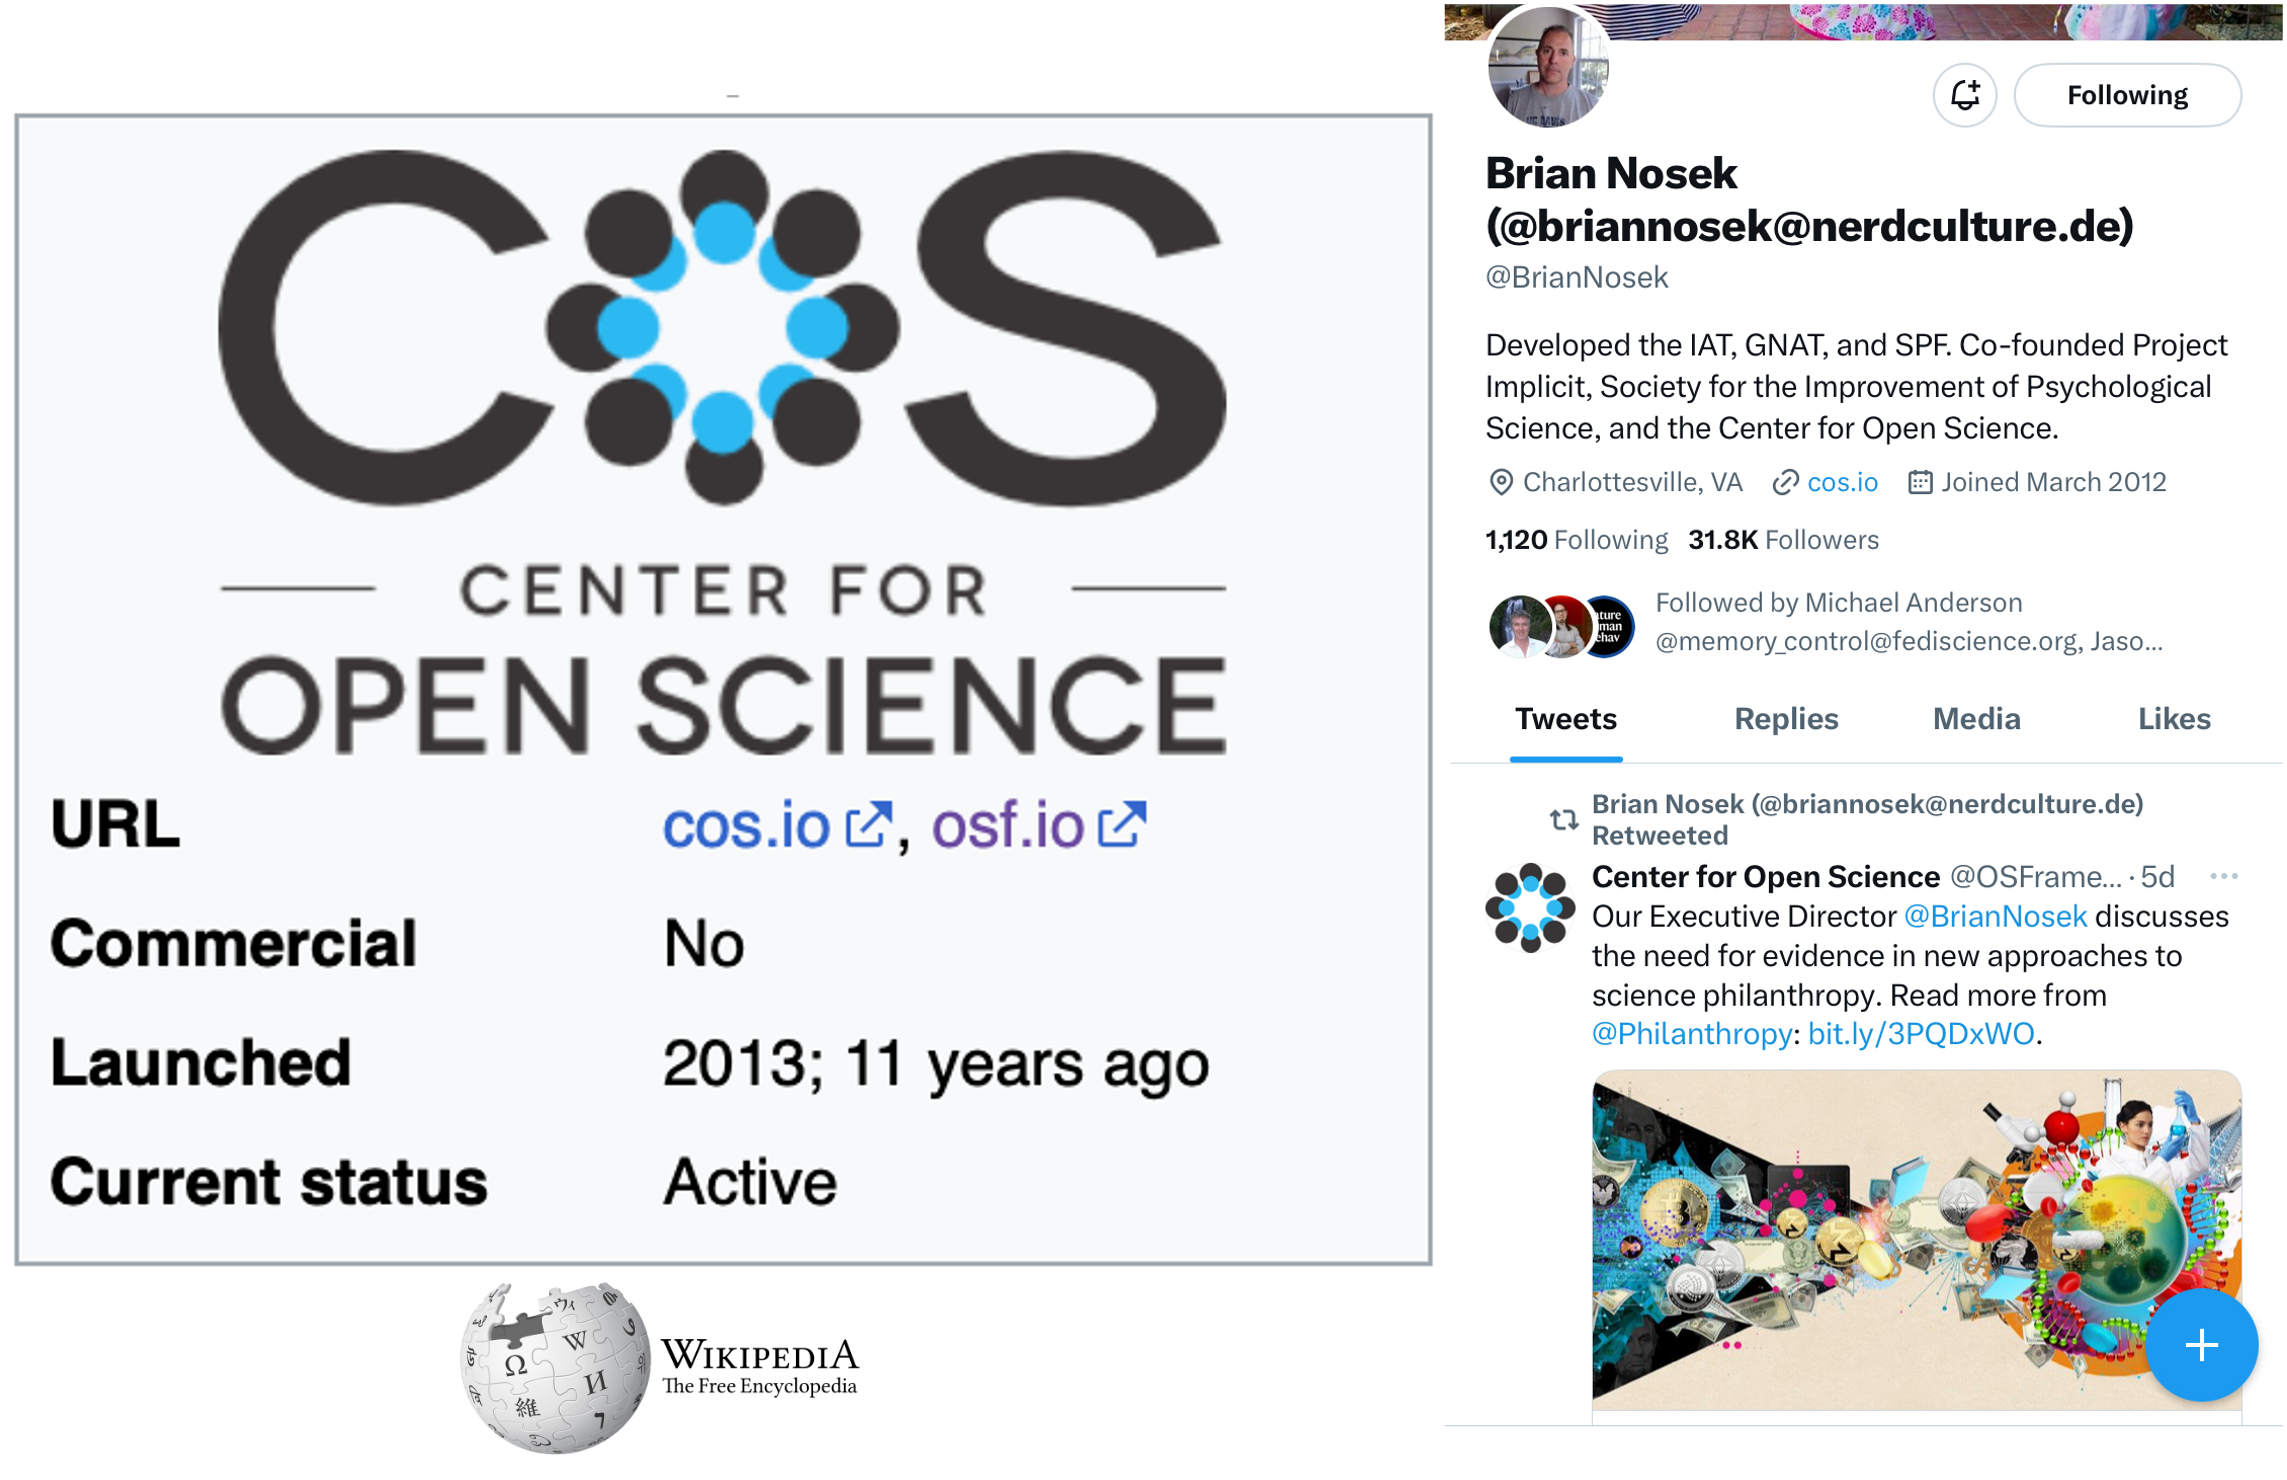
\includegraphics{figs/cos.png}
\end{center}
\end{frame}

\begin{frame}{Open Science Framework}
\phantomsection\label{open-science-framework}
\begin{center}
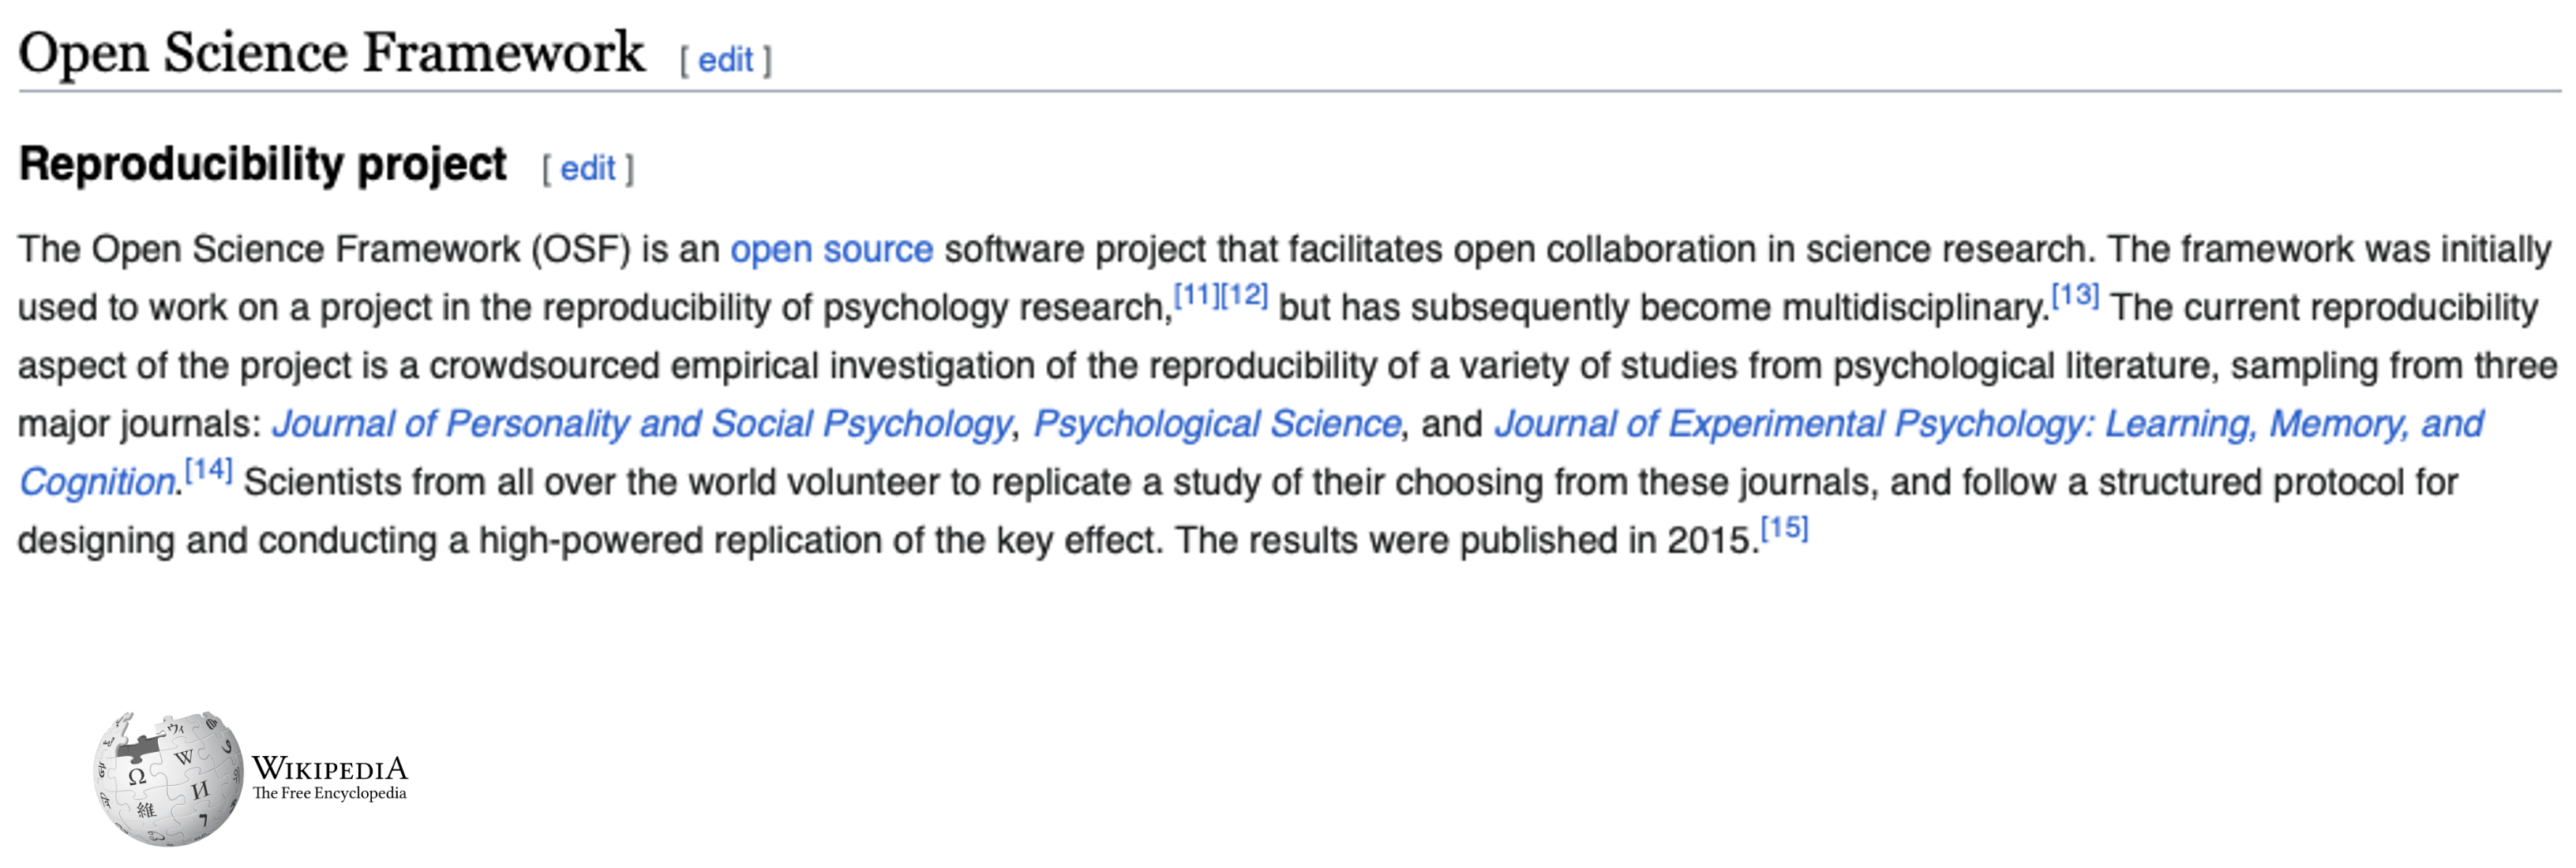
\includegraphics{figs/osf.png}
\end{center}
\end{frame}

\section{Preregistration}\label{preregistration-1}

\begin{frame}{How to Preregister?}
\phantomsection\label{how-to-preregister}
\begin{itemize}
\tightlist
\item
  Various platforms: \url{https://aspredicted.org}, \url{https://osf.io}
\item
  Information to provide: Hypothesis, Dependent variable, Conditions,
  Analyses, Outliers and Exclusions, Sample size, Other.
\item
  Example: \url{https://osf.io/7ghcz}
\end{itemize}
\end{frame}

\begin{frame}{Details}
\phantomsection\label{details}
\begin{itemize}
\tightlist
\item
  \textbf{Hypothesis.} What's the main question being asked, or
  hypothesis being tested in this study?
\item
  \textbf{Dependent variable.} Describe the key dependent variable(s)
  specifying how they will be measured.
\item
  \textbf{Conditions.} How many and which conditions will participants
  be assigned to?
\item
  \textbf{Analyses.} Specify exactly which analyses you will conduct to
  examine the main question/hypothesis.
\item
  \textbf{Outliers and Exclusions.} Describe exactly how outliers will
  be defined and handled, and your precise rule(s) for excluding
  observations.
\item
  \textbf{Sample Size.} How many observations will be collected or what
  will determine sample size?
\item
  \textbf{Other.} Anything else you would like to pre-register? (e.g.,
  secondary analyses, variables collected for exploratory purposes,
  unusual analyses planned?)
\end{itemize}
\end{frame}

\begin{frame}{Preregistration FAQ's}
\phantomsection\label{preregistration-faqs}
\begin{itemize}
\tightlist
\item
  \textbf{After running preregistered analyses, discover something
  surprising!}
\item
  \emph{Totally fine to run exploratory follow-up analyses}
\item
  \emph{Label them as exploratory in the paper}
\item
  \textbf{Learn better analysis technique after study is preregistered}
\item
  \emph{Disclose in paper}
\item
  \emph{Usually, should also run planned analyses}
\item
  \emph{Reporting in supplemental materials okay}
\item
  \emph{If you don't run, need to explain why}
\item
  \textbf{Data already collected}
\item
  \emph{OK to preregister late, but\ldots{}}
\item
  \emph{Ideal to preregister before collection}
\item
  \emph{Important to preregister before looking at data}
\item
  \emph{Vital to preregister before running focal test}
\end{itemize}
\end{frame}

\begin{frame}{Preregistration FAQ's}
\phantomsection\label{preregistration-faqs-1}
\begin{itemize}
\tightlist
\item
  \textbf{Data collection doesn't go as planned}
\item
  \emph{Power analysis indicates n = 200 N are needed to detect our
  effect with 80\% power. We will collect n = 200.''}
\item
  \emph{n = 87 participants failed inclusion criteria}
\item
  \emph{What do you do?}
\item
  \emph{Make reasonable decision, and disclose}
\item
  \textbf{Vague analyses}
\item
  \emph{``ANOVA will test the difference between conditions''}
\item
  \emph{Hypothesized direction of differences?}
\item
  \emph{Post hoc comparisons? Planned comparisons? Which type?}
\item
  \emph{Disclose decision-process, be more specific in future}
\item
  \textbf{Vague hypothesis}
\item
  \emph{``We predict that people will report lower levels of free will
  in A and B conditions than in C condition, and furthermore that free
  will will be lower in the A condition than in B condition.''}
\item
  \emph{What does this predict? A \textgreater{} B \textgreater{} C: (A
  \& B) \textgreater{} C, A \textgreater{} B}
\end{itemize}
\end{frame}

\begin{frame}{A small diversion}
\phantomsection\label{a-small-diversion}
\begin{itemize}
\tightlist
\item
  Predatory journals
\item
  Cloned journals
\end{itemize}
\end{frame}

\section{Conclusion}\label{conclusion}

\begin{frame}{}
\phantomsection\label{section-3}
\end{frame}

\begin{frame}{Some useful references:}
\phantomsection\label{some-useful-references}
\begin{itemize}
\tightlist
\item
  \emph{p}-Hacking: Crash Course Statistics \#30:
  \url{https://youtu.be/Gx0fAjNHb1M}
\item
  The Replication Crisis: Crash Course Statistics:
  \url{https://youtu.be/vBzEGSm23y8}
\item
  Falsification:
\item
  Academic misconduct:
\end{itemize}
\end{frame}

\begin{frame}{}
\phantomsection\label{section-4}
\textbf{Any questions?}
\end{frame}

\begin{frame}{References}
\phantomsection\label{references}
\phantomsection\label{refs}
\begin{CSLReferences}{1}{0}
\bibitem[\citeproctext]{ref-simmons2011}
Simmons, Joseph P., Leif D. Nelson, and Uri Simonsohn. 2011.
{``False-Positive Psychology.''} \emph{Psychological Science} 22 (11):
1359--66. \url{https://doi.org/10.1177/0956797611417632}.

\end{CSLReferences}
\end{frame}



\end{document}
